\documentclass[times]{elsarticle}
\bibliographystyle{elsarticle-num}
\usepackage{graphicx,colordvi}
\usepackage{bm}

\begin{document}
\begin{frontmatter}

\title{LFRic and PSyclone: Building a Domain Specific Language for Weather and Climate models}

\author[met]{S.~Adams}
\author[hartree]{R.~Ford}
\author[met]{M.~Hambley}
\author[met]{J.M.~Hobson}
\author[met]{I.~Kavcic}
\author[met,read]{C.~M.~Maynard}
\ead{c.m.maynard@reading.ac.uk}
\author[met]{T.~Melvin}
\author[bath]{E.H.~Mueller}
\author[met]{S.~Mullerworth}
\author[hartree]{A.~Porter}
\author[downunder]{M.~Rezny}
\author[met]{B.~Shipway}
\author[met]{R.~Wong}




\address[met]{Met Office, FitzRoy Road, Exeter, EX1 3PB}
\address[read]{Department of Computer Science, Polly Vacher Building,
  University of Reading, Reading, UK, RG6 6AY}
\address[bath]{Department of Mathematics, University of Bath, Bath}
\address[downunder]{Monash University, Melbourne, Australia}
\address[hartree]{Hartree Centre, STFC Daresbury, Grim up North}

\begin{abstract}
\end{abstract}

\begin{keyword}

\end{keyword}

\end{frontmatter}

\section{Introduction}
In common with many science applications, Exascale computing presents
a disruptive change for weather and climate models. However, the
difficulty in porting and optimising legacy codes to new hardware is
particular acute for this domain as the software is large ($O(10^6)$
lines of code), takes a long time develop (a decade or more for a new
dynamical core) and is long-lived (typically quarter of a century or longer). These
timescales are much longer than the changes in both processor
architectures and programming models necessary to exploit these
architectures~\cite{gmd-2017-186}. Moreover, highly scalable
algorithms are necessary to exploit the necessary degree of
parallelism Exascale computers are likely exhibit.

In collaboration with academic partners, the Met Office is developing
a new dynamical core, called GungHo~\cite{MELVIN2018342}. By
employing a mixed Finite Element Method on an unstructured mesh, the
new dynamical core is designed to maintain the scientific accuracy of
the current Unified Model (UM) dynamical core (ENDGame~\cite{QJ:QJ2235}),
whilst allowing improved scalability by avoiding the singular pole of
the lon-lat grid. A new atmospheric model and software infrastructure,
named LFRic after Lewis Fry Richardson, is being developed to host the
GungHo dynamical core, as the structured, lon-lat grid is inherent in the
data structures of the UM.

The software design is based on a layered architecture and a 
{\em separation of concerns} between the natural science code in which
the mathematics is expressed and the computational science code where the
parallelism and other performance optimisations are expressed. In particular,
there are three layers. The top layer, the algorithm layer, is where high-level mathematical 
operations on global fields are performed. The bottom layer is the kernel layer
where these operations are expressed on a single column of data. In between is the
Parallelisation System or PSy layer, where the horizontal looping and parallelism is
expressed. This abstraction, called PSyKAl, is written in Fortran with Fortran 2003
Object Orientation to encode the rules of the API.
Moreover, a Python code called Psyclone can parse the algorithm and kernel layers and
generate the Psy layer with different target programming models. In effect, the PSyKAl API
and Psyclone are a Domain Specific Embedded Language (DESL). Natural science code which
conforms to this API can be written in serial and the parallel code is then generated automatically.

The model is under active development and indeed, the science and
numerical analysis are still areas of active research. However, in
order to assess the scientific performance of the model, sufficiently
computationally challenging problems must be tackled. Thus, the
ability to generate optimisations for current architectures is also
required. 

The paper is organised as follows, the GungHo dynamical core and
computational aspects are presented in section~\ref{sec:GH}. The
software design for the separation of concerns and PSKAl API are described 
are described in section~\ref{sec:SoC}. The model infrastructure and
use of libraries is discussed in section~\ref{sec:lib}. PSyclone, the
code generator is presented in section~\ref{sec:Psyclone}. Finally a
scaling analysis is presented in section~\ref{sec:scal} and
conclusions drawn in section~\ref{sec:con}.

\section{\label{sec:GH}GungHo}
A bit about GungHo, but mostly the unstructured mesh, quads, 2+1D
mesh, vertically structured. Etc.

\begin{itemize}
\item 2D Mesh
\item 2D + 1D extrusion, indirection
\item equations
\item mixed fem
\item fv advection
\item timestepping
\item um physics
\end{itemize}

The GungHo dynamical core was developed to replace the current ENDGame
dynamical core in the UM. The GungHo model seeks to replicate the 
accuracy of ENDGame whilst replacing the regular latitude-longitude
grid with a quasi-uniform mesh and so avoid the problems associated with
the polar singularities on in ENDGame and the resulting convergence of 
meridians at the poles. The mesh used in GungHo is an equi-angular
cubed-sphere, Figure \ref{fig:cubed=sphere}, this has the benefit of near
uniform resolution across the globe achieved by using quadrilateral cells. 
However, this quasi-uniform mesh comes as the expense of losing orthogonality
(the line between two neighbouring cells centers is not, in general, 
perpendicular to the edge shared between the two cells. Additionally the 
two polar singularities of the latitude longitude mesh have been replaced 
by the eight corners of the cubed sphere where only three cells meet at a
vertex instead of the usual four. The lack of orthogonality and the presence
of the corner singularities needs to be taken into account when choosing an 
appropriate numerical method.
%
\begin{figure}
\centering\includegraphics[width=0.8\linewidth]{Cubed-Sphere.pdf}
\caption{\label{fig:cubed=sphere} Equi-angular cubed-sphere mesh with 
$12x12$ subdivisions per face, referred to as a $C12$ mesh. This gives 
$864$ columns of cells. }
\end{figure}
%

\textbf{This Section may be better off in the infrastructure part?}
To generate the 3D mesh this 2D mesh is extruded in the radial direction
to form a spherical shell of cells. Where orography is present a terrain
following radial coordinate is used such that every column contains the
same number of cells. The horizontal mesh is treated as unstructured,
such that it could easily be changed, such as to a icosahedral mesh, if
required. The vertical is structured and directly addressed, so that
a data point is addressed as \textit{map(df,col)+k}, where \textit{col}
is the horizontal index of the column and \textit{k=0,...,nlayers-1} is
the index of the vertical layer, \textit{df} is the index of a particular
data point within the cell, allowing multiple data points within a single cell, 
finally \textit{map} is an array containing the address of data points at the bottom of 
the model column.
Using an extruded mesh of this type with direct access in the vertical, the cost
of the indirectly addressed horizontal index can be hidden \citet{gmd-9-3803-2016}.
%

The GungHo dynamical core solves the Euler equations for a perfect gas in a rotating frame
%
\begin{eqnarray}
\frac{\partial\mathbf{u}}{\partial t} & = & -\left(2\bm{\Omega}+\nabla\times\mathbf{u}\right)\times\mathbf{u} - \nabla\left(\frac{1}{2}\mathbf{u}\cdot\mathbf{u} + \Phi\right) - c_p\theta\nabla\Pi,\label{eq:momentum}\\
\frac{\partial\theta}{\partial t} & = & - \mathbf{u}\cdot\nabla\theta,\label{eq:energy}\\
\frac{\partial\rho}{\partial t} & = & - \nabla\cdot\left(\mathbf{u}\rho\right)\label{eq:continuity}.
\end{eqnarray}
%
the system is closed by the equation of state
%
\begin{equation}
\Pi^{\frac{1-\kappa}{\kappa}} = \frac{R}{p_0}\rho\theta.\label{eq:eos}
\end{equation}
%
These constitute a set of coupled nonlinear pdes for the vector wind $\mathbf{u}$, 
the density $\rho$, potential temperature $\theta$ and Exner pressure $\Pi$. 
Additionally $\bm{\Omega}$ is the rotation rate, $\Phi$ is the geopotential, $p_0$ is a reference pressure, $R$ is the 
gas constant, $c_p$ is the specific heat at constant pressure and $\kappa\equiv R/c_p$.

In order to maintain a similar
accuracy to ENDGame on a quasi-uniform mesh a mixed finite element method is used \citep{cotter2012, natale2016},
this gives the finite element equivalent of the C-grid Charney-Philips staggering
used in ENDGame. The mixed finite element method involves defining a number
of finite element spaces and mappings between them. The particular family of spaces \citep{boffi2013} used in
 GungHo, for a given polynomial order $l$, are: $Q_{l+1}$ containing continuous 
point wise scalar quantities; $N_l$ containing circulation vectors that have
continuous tangential components; $RT_l$ containing flux vectors that have 
continuous normal components; $Q_l^D$ containing discontinuous volume 
integrated scalars; along with a horizontally discontinuous vertically continuous space
for $\theta$ \citep{natale2016} to mimic the Charney-Philips grid staggering used in ENDGame. 
In practice the lowest order spaces $l=0$ are used. 
See \citet{melvin2018} for a full description of the discretisation used in the GungHo 
model.

As in ENDGame, to facilitate the use of long timesteps a iterative semi-implicit
timestepping scheme is used, this requires within each timestep a nonlinear Picard
iteration to update the nonlinear and advection terms and at each Picard iteration
a large sparse linear system is solved, which is formed by use of a quasi-Newton method,
%
\begin{equation}
\mathcal{L}\left(\mathbf{x}^n\right)\mathbf{x}' = \mathcal{R}\left(\mathbf{x}^{(k)}\right),\label{eq:quasi-newton}
\end{equation}
%
For the increment $\mathbf{x}'\equiv\mathbf{x}^{(k+1)}-\mathbf{x}^{(k)}$ on the $k^{\rm{th}}$ 
estimate from the Picard iteration of the prognostic variables $\mathbf{x}\equiv\left(\mathbf{u},\,\theta,\,\rho,\,\Pi\right)$. The linear system $\mathcal{L}\left(\mathbf{x}^n\right)$ is chosen as to contain the terms necessary for stability of the fast acoustic and gravity waves as in \citet{QJ:QJ2235} and is formed from a linearisation about the previous timestep fields $\mathbf{x}^n$. The method used to solve this linear system is detailed in Section \ref{sec:Solver}.





\section{\label{sec:SoC}Separation of Concerns}
Science applications in general and weather and climate codes in
particular are written in high-level languages such as Fortran or
C/C++. Indeed, Fortran is commonly employed for weather and climate
codes and can be considered a Domain Specific Language (DSL) for
numerical computation. Using a such a high-level language, an
algorithm is written to solve a mathematical problem without
consideration for the processor architecture. The compiler generates
machine specific instructions and can, in principle, make optimisation
choices to exploit the architecture of different processors.

This abstraction of a separation of concerns between mathematics code
and machine code is powerful and enables both the portability of
science code to different processor architectures and allows the
application to exploit a significant\footnote{What constitutes good
  performance depends on a variety of factors.} fraction of the peak
performance of the processor. Whilst many science applications may
contain code optimisations in performance critical sections, for
example, blocking or tiling loop nests to better utilise cache memory,
in general these applications have relied on clock
speed increases between processor generations to increase performance.

Processor speed increases between generations ceased more than a decade
ago due to the absence of Dennard scaling~\cite{dennard}. Instead,
successive generations of processors have had increasing numbers of processor cores per
socket. Science applications have already been adapted to run on multiple
nodes to exploit supercomputers with the distributed memory, data parallelism
typical expressed over MPI. However, multi-core nodes present
additional challenges and heterogenous compute nodes such as
CPU + GPU with distinct memory spaces require additional programming
models. Moreover, the algorithms employed combined with data
parallelism may not be sufficient to exploit this explosion of parallelism.

Many programming models exist, MPI and Partitioned Global Address
Space (PGAS) languages, such as Co Array Fortran, Unified Parallel C,
Chapel and GASPI for distributed memory, new programming languages such
as OpenCL or CUDA and directive based programming models for threaded
and shared memory parallelism such as OpenMP or OpenACC. However,
the programming models lag behind in development of the rapidly evolving computer
architectures and particular models lack feature or processor coverage
making the choice of programming model difficult. This is especially
problematic for weather and climate applications with their long development
cycles. 

Many applications have adopted an MPI + X model, where X is one or
more of the programming models mention in the previous paragraph. This
is problematic for several reasons. The programming models are not
only different, they are different types of model. Languages, language
extensions, libraries and directives, some of which are architecture
specific. Worse, the interaction between them is outside the scope of
any model\footnote{Whilst MPI has some level of threaded awareness,
  this is limited.} and may, for example, require the batch scheduling
system to control this. The applications may require a different X for
different architectures and even different data layouts and
loop nest order. All these parallel and performance features
break the data abstraction of the separation of concerns between the
maths/science code and architecture specific code.

The design for the LFRic model is based upon computational science
report from phase 1 of the GungHo project~\cite{GHP1_CSR}. By
employing a layered software architecture, the complex parallel code
code can be kept separate from the science code. The software is
separated into three layers. The top layer is the algorithm
layer. Here, algorithms are expressed as operations on global,
data-parallel field objects. The middle layer, termed the
Parallelisation System or PSy layer contains the horizontal looping
and is where the data parallelism is expressed.  The bottom layer is
comprised of the kernels which encode the operation invoked in the
algorithm layer. These operate on a single column of data. 
Shown in figure~\ref{fig:psykal} is a schematic diagram of this
layered software achitecture. The red arrows indicate the control flow
though the different layers. 

\begin{figure}
\centering\includegraphics[width=0.8\linewidth]{PSyKAl.pdf}
\caption{\label{fig:psykal} Schematic diagram of the PSyKAl layered
  architecture. A single model could be for example, the atmospheric
  model. The blue vertical line between the PSy layer and the
  Algorithm and Kernel layers represents a separation of the science
  and parallel code.}
\end{figure}

The APIs between the layers are tightly controlled. The PSy layer can
only be called from the algorithm layer by an {\em invoke} procedure
call. The permitted arguments to these invoke prodecures are resticted
to be the kernels and the fields that the kernels will operate on. The
kernels can only be called from the PSy layer with the unpacked data
arrays, scalars for loop bounds and supporting arrays of both reals
and integers for Finite Element Method over an unstructured mesh.
These coding rules are enforced by using Fortran 2003 object
orientation style to control the APIs. By restricting the domain of
the problem from all numerical mathematics to only that required (in
the first instance) to the GungHo dynamical core it is possible to
constrain the parallelism to the PSy layer. By restoring the
separation of concerns between the science code and the
parallel/optimisation code means in principle different programming
models can be employed in the PSy layer without changing the science
code. Moreover, the PSyKAl API can be thought of a Domain Specific
Embedded Language (DSEL).

Compilers in general have to be conservative about the assumptions
they can make in order to guarantee correctness. However, a further
advantage of the domain specific approach is that developers can
explicitly express the domain knowledge which is not possible in a
standard, high level language. In the case of the LFRic model, data
access descriptors are employed to say whether access to a field is
read, write, readwrite or increment. This information is embedded in
Fortran as part of the kernel. Other information encoded in this way
is the loop iterator (for example {\em cells}), whether the kernel
operates on a field which lives on a specific function space, whether
any of the fields live on common function spaces and for FEM kernels
whether the kernel uses any basis functions. 

The restricted domain, strict control of the APIs between layers and
critically, the data access descriptors and other kernel metadata
allow the PSy layer to be constructed entirely according to a set of
rules. The code itself can then be automatically generated. This is
done by a python code parser, transformer and code generator called
PSyclone. More details of PSyclone itself can be found in
section~\ref{sec:psyclone}. The generated code is mostly Fortran.
These are calls to the LFRic infrastructure which might contain the MPI
distributed memory parallelism and calls to the LFRic infrastructure to dereference the Fortran 2003
objects, looping over the horizontal mesh elements and calling the
kernels themselves. However, PSyclone can also perform transformations
and target other progamming models such as OpenMP or OpenACC. PSyclone
is then in effect a DSEL compiler. PSyclone also does one other
important code generation function. In the algorithm layers, the calls
to the invoke procedure are replaced with a specific prodcedure call
to the PSy layer. The PSy layer code can then be optimised depending on
the kernels in the invoke and the metadata. 

\section{\label{sec:lib}Infrastructure}.
ESMF, YAXT, XIOS, pFunit? netcdf etc.

\section{\label{sec:psyclone}PSyclone}.
The code generator.

\section{\label{sec:Solver}Linear solvers and preconditioners}
Iterative solvers for large sparse linear systems of equations are
required in several places in the model. For example, since mass
matrices in the finite element discretisation are not diagonal, they
need to be inverted with a small number of iterations of a Krylov
subspace method. More importantly, the semi-implicit time-stepping
approach requires the solution of a very large sparse system for all
prognostic unknowns in each step of the non-linear Picard
iteration. Since the system is ill-conditioned, it needs to be
preconditioned efficiently. This is achieved by the (approximate)
reduction to an elliptic system for the pressure, which is
preconditioned with a tensor-product multigrid algorithm
\cite{Borm2001} (see Section \ref{sec:preconditioner}). To increase
efficiency, the pressure preconditioner can be wrapped in its own
iterative solver for the Helmholtz system. Note that in contrast to
the approach already employed in the ENDGame model \cite{QJ:QJ2235},
an outer iteration over the full system is still required due to the
non-diagonal nature of the finite element mass matrices. Altogether
this results in a rather complex solver.
\subsection{Solver infrastructure}
To allow easy implementation of sophisticated nested iterative solvers
and preconditioners, a dedicated abstraction was developed by using
advanced object oriented features of Fortran 2003. This approach
follows similar design philosophies in widely used linear algebra
libraries such as PETSc \cite{Balay1997,Balay2018} and DUNE-ISTL
\cite{Blatt2007}. More specifically, the implementation in LFRic uses
derived types which realise the following operations (see
Fig. \ref{fig:class_hierarchy}, left):
\begin{itemize}
\item \textbf{Vector} types which support common linear algebra
  operations such as AXPY $y\mapsto y+\alpha x$ and dot products
  $x,y\mapsto s = \langle x,y\rangle$. The most important vector-type
  is \texttt{field\_vector}, which contains a collection of model
  fields.
\item \textbf{Linear operator} types which implement the operation $x\mapsto y=Ax$ for vectors $x$ and $y$
\item \textbf{Preconditioners} which approximately solve the system $Px=b$ for a
  given right hand side $b$ and some operator $P\approx A$
\item \textbf{Iterative solvers} which solve the system $Ax=b$ with a
  Krylov-subspace method for a given right hand side $b$. Currently
  supported solvers include Conjugate Gradient, GMRES and BiCGStab.
\end{itemize}
\begin{figure}
  \begin{center}
    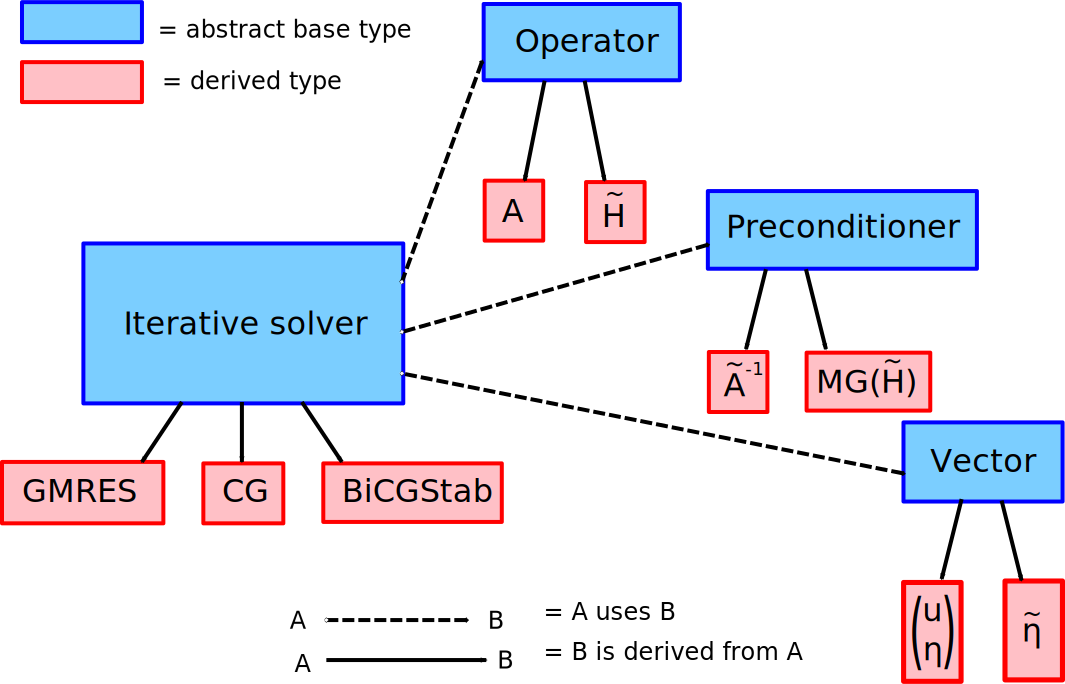
\includegraphics[width=0.45\linewidth]{class_hierarchy.pdf}
    \hfill
    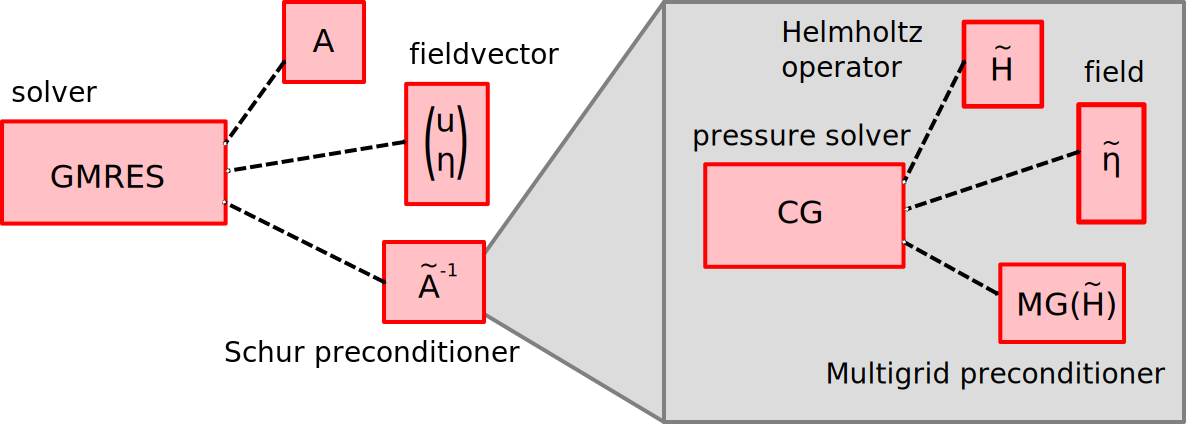
\includegraphics[width=0.45\linewidth]{class_concrete.pdf}
    \caption{Derived class hierarchy for solvers and preconditioners
      in LFRic (left) and concrete implementation for the linear
      system in implicit time-stepping (right).}
    \label{fig:class_hierarchy}
  \end{center}
\end{figure}
Each of those types is derived from an abstract base type. The
iterative solver types operate on generic vector types and are passed
preconditioner and linear operator objects which adhere to the
interface of their abstract base types.  This implies that only one
instance of a particular Krylov method has to be implemented in the
code. Apart from avoiding code duplication, this increases reliability
and maintainability, since only one instance of each solver has to be
developed and tested. In addition, it allows easy ``plug-and-play'' to
explore the space of all possible solver/preconditioner combinations
to achieve optimal performance.

To solve a particular problem, the user has to develop bespoke derived
types for the corresponding linear operator and preconditioners. Note
that the \texttt{apply()} methods of those derived types contain
invoke kernels, which guarantees optimal performance of the entire
model. For example, to construct a solver for the implicit linar
system which is inverted in every semi-implicit time-step, the user
implements the following objects (see Fig. \ref{fig:class_hierarchy},
right):
\begin{itemize}
\item A linear operator type which applies the full linear system to
  all components of a \texttt{field\_vector}.
\item A preconditioner type which reduces the full linear system to
  the (approximate) Schur complement in pressure space by lumping the
  velocity mass matrix; this preconditioner then calls the solver for
  the pressure (Helmholtz-) system.
\item A linear operator type which applies the Helmholtz-operator for
  the pressure system.
\item A preconditioner type which approximately inverts the Helmholtz
  operator (see section \ref{sec:preconditioner}).
\end{itemize}
Once implemented, those linear operators/preconditioners need to be
passed to suitable existing linear solvers.

In addition to this more traditional approximate Schur-complement
approach for solving the full linear system, the development of
solvers based on a hybridisation approach is currently explored. Since
an exact Schur-complement can be formed in this case, hybridisation
avoids the expensive iteration over the full linear system, and
potentially leads to significant improvements in performance.
\subsection{\label{sec:preconditioner}Preconditioner}
To precondition the strongly anisotropic Helmholtz-operator for the
pressure system, the tensor-product multigrid approach in
\cite{Borm2001} is used in LFRic. This is a more advanced solver than
the current tridiagonal vertical-only preconditioner in the ENDGame
model. The multigrid algorithm used in LFRic has been tested
extensively for representative elliptic equations in atmospheric
modelling in \cite{Mueller2014,Dedner2016}, including a mixed-finite
element discretisation of a linear gravity wave system in
\cite{Mitchell2016}. The key idea to address the strong vertical
anisotropy due to the high-aspect ratio of the domain is to combine
vertical-only smoothing (line relaxation) with a horizontal multigrid
hierarchy. To allow the easy construction of the vertical-only
operators in the Schur-complement from the finite element
discretisation of the full equations, a suitable operator algebra was
developed in \cite{Mitchell2016} and tested in the Firedrake
library. For horizontally discontinuous function spaces (such as the
pressure space and the vertical-only velocity), operators can be
assembled into a partially assembled matrix type, which stores all
couplings within one vertical column. Matrices of this type can be
multiplied, added and, most importantly, inverted in the tridiagonal
solvers which realises the vertical line relaxation. This allows the
high-level construction of the building blocks required for the
Helmholtz-solver and preconditioner. The same data structures were
implemented as derived Fortran 2003 types in the LFRic code and form
the building blocks of the tensor-product multigrid preconditioner for
the elliptic Helmholtz system.

Compared to simpler preconditioners, which do not combine vertical
line relaxation with a horizontal multigrid hierarchy, the
tensor-product multigrid approach typically reduces the solution time
of the pressure system by a factor of at least two
\cite{Mueller2014,Mitchell2016}. However, since the Helmholtz system
contains a zero-order term, only a small number ($\approx 3-4$) of
multigrid levels is required (independent of the grid
resolution). This greatly increases scalability since it avoids global
couplings which arise on the coarsest level.

\section{\label{sec:scal}Scaling}.
Scaling, MPI and OpenMP etc.

\section{Conclusion}
\label{sec:con}
Conclusions, future work etc


\bibliography{mibib.bib}

\end{document}
